\documentclass[12pt, a4paper]{article}


%%%% Encodings

\usepackage[utf8]{inputenc} % encoding
\usepackage[english]{babel} % use special characters and also translates some elements within the document.

%%%% Misc

\usepackage{hyperref}[colorlinks=true, urlclor=blue]       % Hyperlinks \url{url} or \href{url}{name}
\usepackage{parskip}        % \par starts on left (not idented)
\usepackage{tocbibind}      % Adds the bibliography to the table of contents (automatically)

% \usepackage[document]{ragged2e}  % Left-aligned (whole document)
% \begin{...} ... \end{...}   flushleft, flushright, center

%%%% Abstract

\usepackage{abstract}       % Abstract

% http://www.ctex.org/documents/packages/special/abstract.pdf
\renewcommand{\absnamepos}{flushleft} % \begin{abstract} \noindent ... \end{abstract}
\setlength{\absleftindent}{0pt}
\setlength{\absrightindent}{0pt}

%%%% Graphics

\usepackage{graphicx}
\graphicspath{{./figures/}} % directory to look up for graphics

% \begin{figure}[h]
%   \centering
%   \includegraphics[scale=0.5]{cat}  % [width=\textwidth, height=4cm],
%   \caption{Example of a cat}
%   \label{fig:cat}
% \end{figure}

%%%% Math

\usepackage{amsmath}        % Math
\usepackage{amssymb}        % New symbols http://milde.users.sourceforge.net/LUCR/Math/mathpackages/amssymb-symbols.pdf
\usepackage{bm}             % $\bm{D + C}$

\usepackage{amsthm} % Math, \newtheorem, \proof, etc
% \begin{theorem}\label{t:label}  ...  \end{theorem}
% \begin{proof} ... \end{proof}
\theoremstyle{plain} % default
\newtheorem{theorem}{Theorem}[section]
\newtheorem{corollary}{Corollary}[theorem]  % Numering depends on the current section (instead of global)
\newtheorem{lemma}[theorem]{Lemma} % Shares numeration with theorem.
\theoremstyle{definition}
\newtheorem{definition}{Definition}[section]
\theoremstyle{remark}
\newtheorem*{remark}{Remark}

% Defines a new environment to write your or claim - proof
\newenvironment{claim}[1]{\par\noindent\underline{Claim:}\space#1}{}
\newenvironment{claimproof}[1]{\par\noindent\underline{Proof:}\space#1}{\hfill $\blacksquare$}

%%%% Code/Pseudo-code

\usepackage{minted} % Code listing
% \mint{html}|<h2>Something <b>here</b></h2>|
% \inputminted{octave}{BitXorMatrix.m}

%\begin{listing}[H]
  %\begin{minted}[xleftmargin=20pt,linenos,bgcolor=codegray]{haskell}
  %\end{minted}
  %\caption{Example of a listing.}
  %\label{lst:example} % You can reference it by \ref{lst:example}
%\end{listing}

\newcommand{\code}[1]{\texttt{#1}} % Define \code{foo.hs} environment

\usepackage[vlined,ruled]{algorithm2e} % pseudo-code http://tug.ctan.org/macros/latex/contrib/algorithm2e/doc/algorithm2e.pdf

%%%% Colors

\usepackage{xcolor}         % Colours \definecolor, \color{codegray}
\definecolor{codegray}{rgb}{0.9, 0.9, 0.9}
% \color{codegray} ... ...
% \textcolor{red}{easily}

%%%% Math

%\makeglossaries % before entries

%\newglossaryentry{latex}{
    %name=latex,
    %description={Is a mark up language specially suited
    %for scientific documents}
%}

% Referene to a glossary \gls{latex}
% Print glossaries \printglossaries

\usepackage[acronym]{glossaries} %

% \acrshort{name}
% \acrfull{name}
% \newacronym{foo}{arcshort}{acrfull}

\usepackage{enumitem} % \begin{enumerate}[label=(\alph*)]

\usepackage{multirow}


\usepackage{fancyhdr}
\pagestyle{fancy}
\fancyhf{}
\lhead{\bf Knowledge Graphs}
\rhead{Arnau Abella, Llu\'is Gr\'ifols}
\lfoot{Open Data}
\rfoot{May 2021}

\title{%
  \vspace{-10ex}
  Knowledge Graphs \\
  \large{Open Data}}
\author{Arnau Abella\\Llu\'is Gr\'ifols}
\date{\today}

\begin{document}

\maketitle

% \vspace{5ex}
\section{Introduction}\label{sec:introduction}

The project is publicly available at \href{https://github.com/monadplus/od-project-3}{Github}.

\section{TBOX definition}\label{sec:tbox}

In order to create our ontology we decided to use \textit{OWL} since our ontology required restrictions which cannot be expressed with \textit{RDFS}.

To model our ontology, we represented the problem statement as a UML diagram (see fig. \ref{fig:uml}) and then we translated this UML to OWL.

\begin{figure}[H]
  \centering
  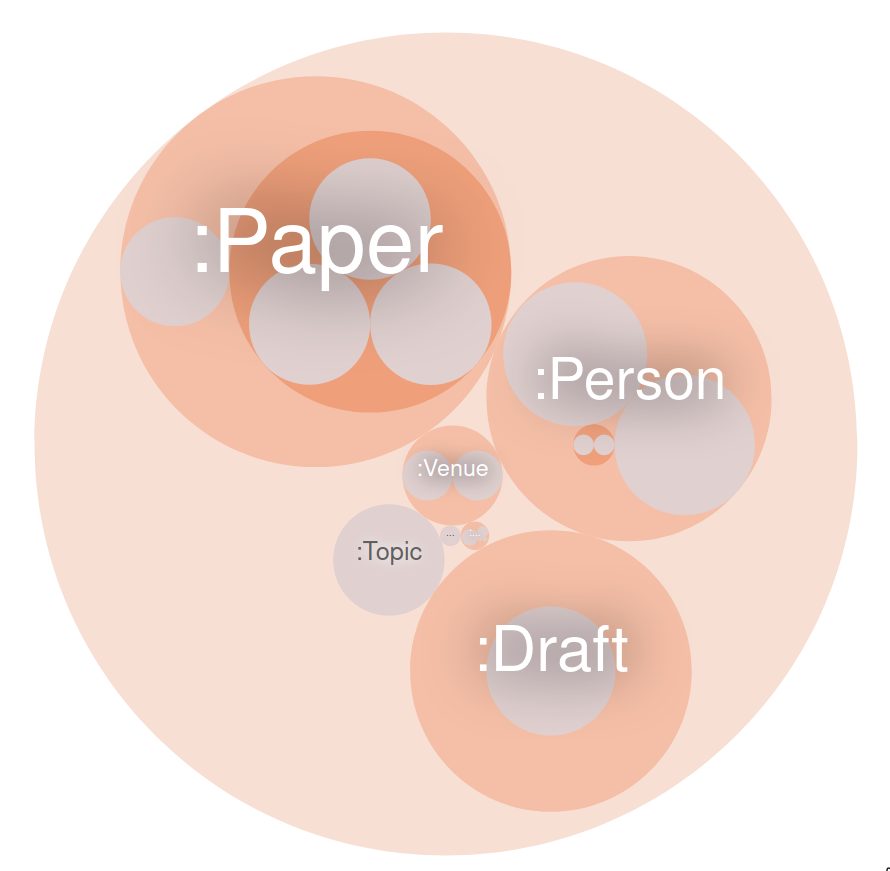
\includegraphics[width=0.5\textwidth]{tbox}
  \caption{TBOX Graph Representation}
  \label{fig:tbox}
\end{figure}

\begin{figure}[H]
  \centering
  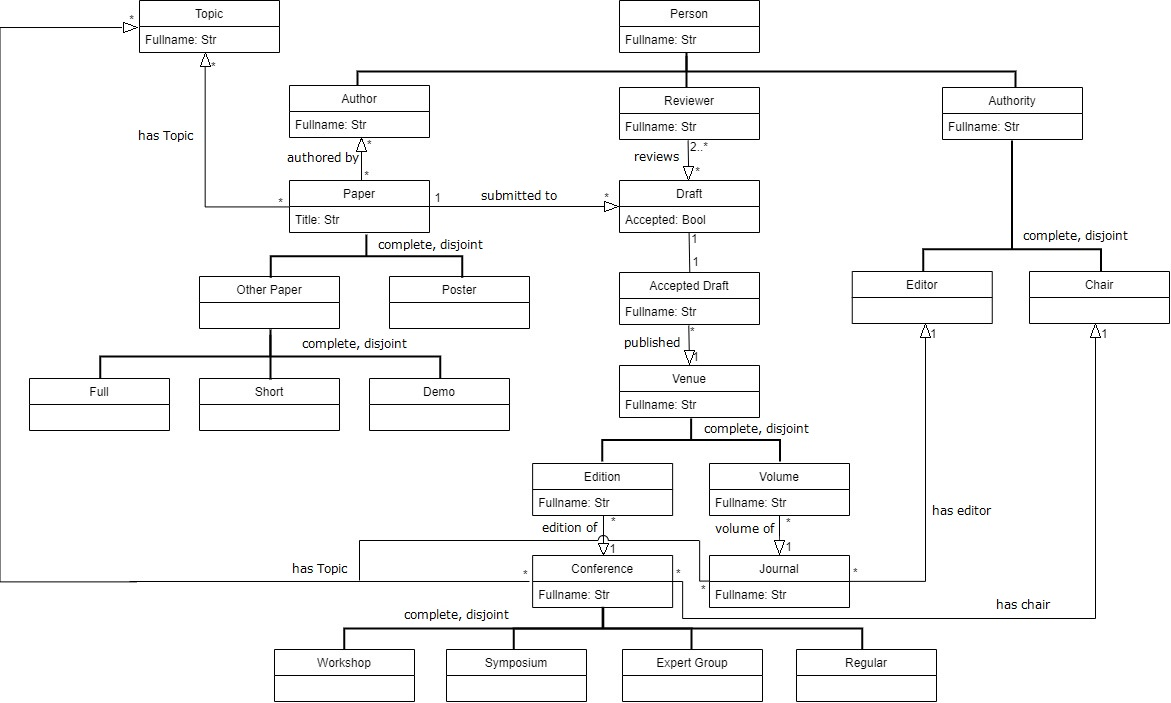
\includegraphics[width=\textwidth]{uml}
  \caption{UML Class Diagram}
  \label{fig:uml}
\end{figure}

For this project, we have used the programming language \textit{Python} and Python's library \textit{Owlready2} \cite{Owlready2}. Owlready2 is an eDSL for Python which translates Python's syntax to OWL's definitions using the following rules:

\begin{itemize}
  \item \code{owl:Class} and \code{rdf:Property} is defined using a python's class definition.
  \item \code{rdfs:subClassOf} and \code{rdfs:subPropertyOf} is defined using Python's inheritance.
  \item \code{owl:ObjectProperty}, \code{owl:DataProperty} and \code{owl:FunctionalProperty} are defined using class inheritance from Python's classes \code{ObjectProperty}, \code{DataProperty} and \code{FunctionalProperty}, respectively.
  \item \code{rdfs:domain} and \code{rdfs:range} is defined using a class attribute.
  \item \code{owl:Restriction} is also defined using a class attribute.
\end{itemize}

\pagebreak

As an example of our ontology, the class \textit{AcceptedDraft} is defined as follows

\begin{listing}[H]
  \begin{minted}[xleftmargin=0pt, breaklines=true, breakanywhere, fontsize=auto]{xml}
<owl:Class rdf:about="#AcceptedDraft">
  <rdfs:subClassOf rdf:resource="#Draft"/>
  <rdfs:subClassOf>
    <owl:Restriction>
      <owl:onProperty rdf:resource="#published"/>
      <owl:onClass rdf:resource="#Venue"/>
      <owl:qualifiedCardinality rdf:datatype="http://www.w3.org/2001/XMLSchema#nonNegativeInteger">1</owl:qualifiedCardinality>
    </owl:Restriction>
  </rdfs:subClassOf>
  <owl:equivalentClass>
    <owl:Class>
      <owl:intersectionOf rdf:parseType="Collection">
        <rdf:Description rdf:about="#Draft"/>
        <owl:Restriction>
          <owl:onProperty rdf:resource="#accepted"/>
          <owl:hasValue rdf:datatype="http://www.w3.org/2001/XMLSchema#boolean">true</owl:hasValue>
        </owl:Restriction>
      </owl:intersectionOf>
    </owl:Class>
  </owl:equivalentClass>
</owl:Class>
  \end{minted}
  \caption{AcceptedDraft Class definition}
  \label{lst:draft}
\end{listing}

The code to generate the ontology and the ontology itself can be found at \code{OD-E\_B1\_AbellaGrifols.py} and \code{OD-E\_B1\_AbellaGrifols.rdf}, respectively.

\section{ABOX definition}\label{sec:abox}

For the ontology's ABOX, we have used data extracted from DBLP \cite{DBLP}. The missing classes such as paper and workshop subtypes were assigned following a normal distribution from a synthetic dataset.

For this part, we have also used Owlready2. Owlready2 has a unique approach to ABOX generation. Once an ontology is loaded into Python's runtime, all elements from the ontology are available as Python's constructs such as classes or class attributes. The user only has to instantiate those classes and attributes in order to generate the corresponding ABOx. For example, a \code{publications:Draft} is instantiated as follows:

\begin{listing}[H]
  \begin{minted}[xleftmargin=20pt,linenos,breaklines=true, breakanywhere, fontsize=auto]{python}
draft = Draft("draft_1")
draft.isReviewedBy = [reviewer1, reviewer2]
draft.supervisedBy = [chair]
draft.accepted = True
draft.published = [volume]
  \end{minted}
  \caption{ABOX programatically definition}
  \label{lst:draft}
\end{listing}

The code and ontology instances for this section can be found at \code{OD-E\_B2\_AbellaGrifols.py} and \code{OD-E\_B2\_AbellaGrifols.rdf}, respectively.

\section{Create the final ontology}\label{sec:create}

An OWL DL reasoner was capable of infering the following knowledge from our ontology:

\begin{itemize}
  \item A Person is infered to be an Author/Reviewer/Editor/Chair depending on the relationship domain/range.
  \item A Venue is infered to be a Conference/Journal depending on the relationship domain/range.
  \item A Draft is infered to be AcceptedDraft depending on the Datatype property 'accepted'.
  \item A Paper is infered to be a Poster if it is presented in a Conference.
  \item Inverse properties such as AuthorOf/AuthoredBy are infered.
\end{itemize}

As an extra, Owlready2 is equipped with a powerful reasoner engine with allowed us to check the correctness of our ontology and to verify if our instances were following the restrictions of our ontology. Owlready2 also provides an SPARQL engine, which combined with the provided reason, the user can test if the ontology is sound and the inference is working as expected.

\begin{table}[H]
  \centering
  \begin{tabular}{ll}
    Number of Classes & 115\\
    \hline
    Number of Properties & 90\\
  \end{tabular}
  \caption{Ontology statistics}
  \label{table:summary1}
\end{table}

We provide a summary table of the resulting knowledge graph (see tables \ref{table:summary1}, \ref{table:summary2.1}, \ref{table:summary3})

\begin{table}[H]
  \centering
  \begin{tabular}{cccc}
    \multirow{4}{*}{Paper}&\multirow{3}{*}{OtherPaper}& Full & 4335\\
    &&Demo & 4198\\
    &&Short & 4292\\
    &  Poster & & 1815\\
    &&& 14640\\
    \hline
    \multirow{4}{*}{Person}&\multirow{2}{*}{Authority}& Chair & 3\\
    &&Editor & 3\\
    & Author & & 20317\\
    & Poster & & 15846\\
    &&&25614\\
    \hline
    \multirow{2}{*}{Venue} & Edition & & 30\\
    & Volume & & 30\\
    && Total Venue &60\\
    \hline
    \multirow{2}{*}{Draft} & AcceptedDraft & & 7283\\
    & && 14640\\
    \hline
    \multirow{4}{*}{Conference} & Regular Conference & & 2\\
    & Expert Group & & 1\\
    & Symposium & & 0\\
    & Workshop & & 0 \\
    &&& 3\\
    \hline
    Journal & & & 3\\
    \hline
    Topic & & & 2139\\
  \end{tabular}
  \caption{Classes breakdown}
  \label{table:summary2.1}
\end{table}

\begin{table}[H]
  \centering
  \begin{tabular}{ll}
    authorOf & 38765 \\
    chairOf & 5\\
    editorOf & 4\\
    draftOf & 14640\\
    responsibleFor & 21960\\
    editionOf & 30\\
    volumeOf & 30\\
    hasTopic & 36629\\
    published & 7283 \\
    reviews & 24808 \\
  \end{tabular}
  \caption{Properties breakdown}
  \label{table:summary3}
\end{table}

\begin{figure}[H]
  \centering
  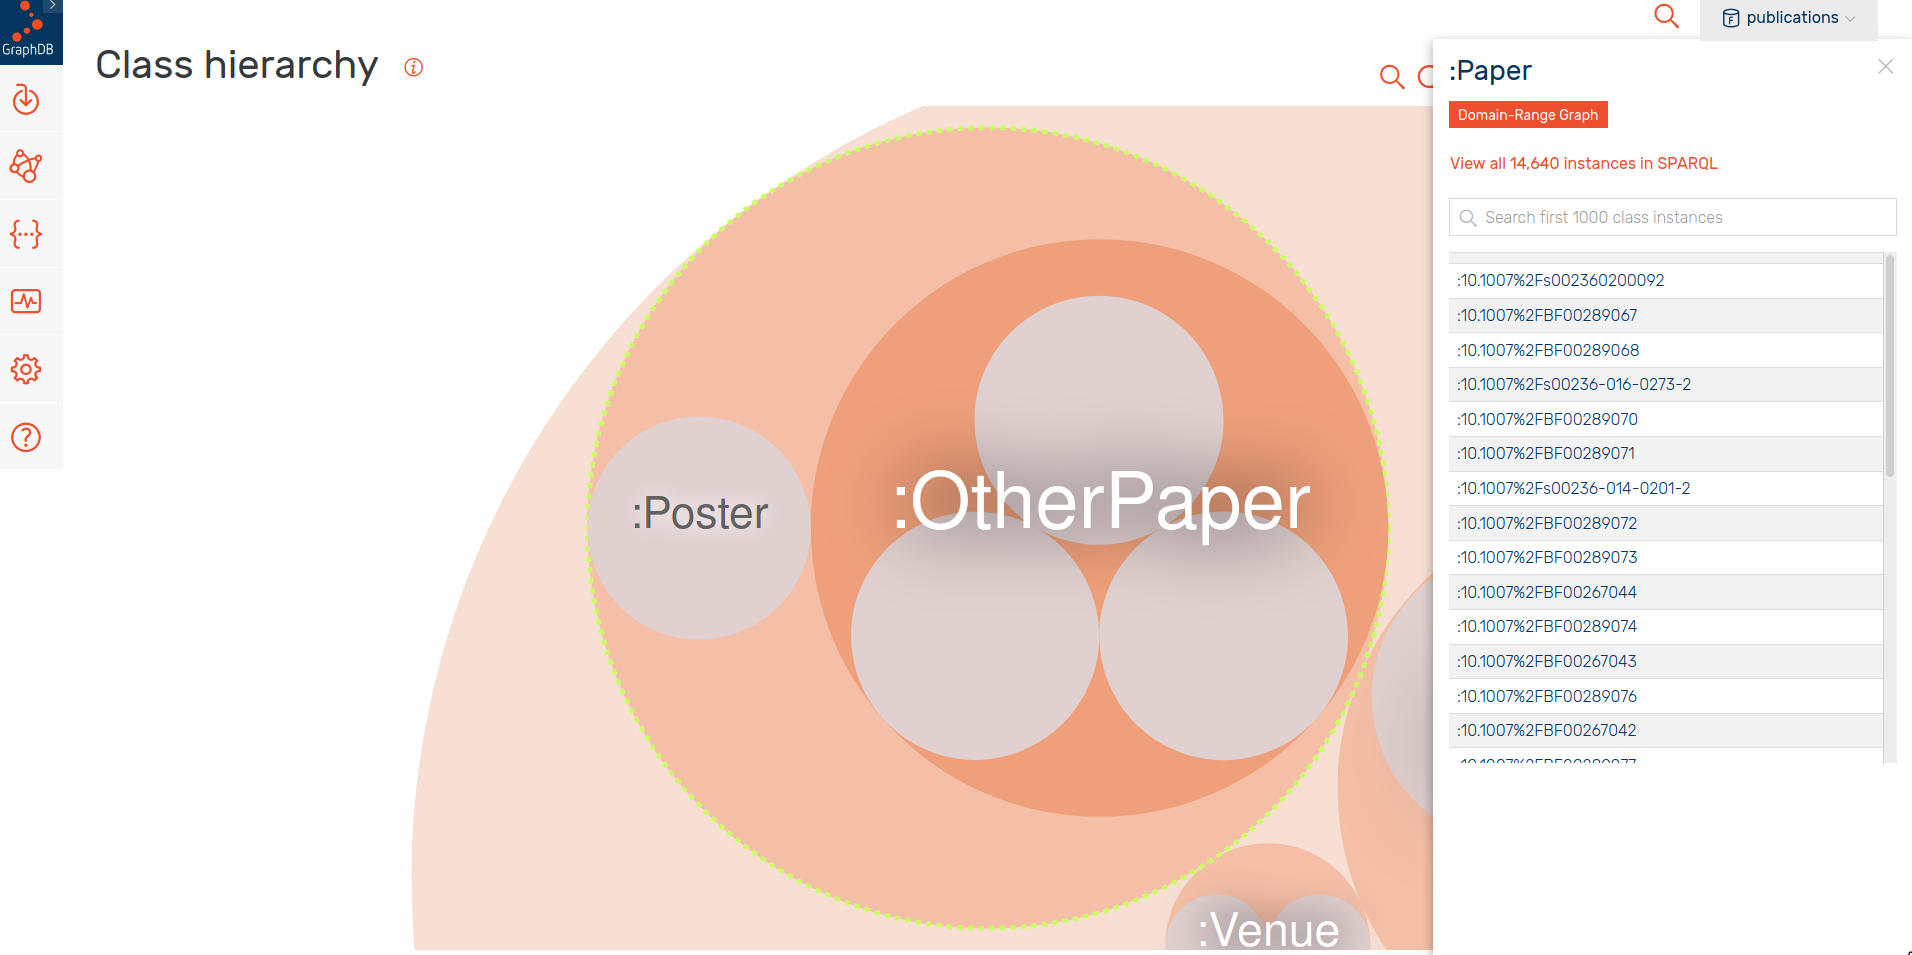
\includegraphics[width=1.2\textwidth]{abox}
  \caption{GraphDB instances}
  \label{fig:abox}
\end{figure}

\section{Querying the ontology}\label{sec:query}

\subsection{Find all Authors}\label{subsec:query1}

\begin{verbatim}
PREFIX : <http://localhost:7200/publications#>

select ?name where {
  ?author a :Author .
  ?author :fullname ?name
} limit 100
\end{verbatim}

\subsection{Find all properties whose domain is Author}\label{subsec:query2}

\begin{verbatim}
PREFIX : <http://localhost:7200/publications#>
PREFIX rdf: <http://www.w3.org/2000/01/rdf-schema#>

select ?p where {
  ?p rdf:domain :Author .
} limit 100

\end{verbatim}

\subsection{Find all properties whose domain is either Conference or Journal}\label{subsec:query3}

\begin{verbatim}
PREFIX : <http://localhost:7200/publications#>
PREFIX rdf: <http://www.w3.org/2000/01/rdf-schema#>

select distinct ?p where {
  {?p rdf:domain :Conference}
  UNION
  {?p rdf:domain :Journal}
} limit 100
\end{verbatim}

\subsection{Find all the papers written by a given author that where published in database conferences}\label{subsec:query4}

\begin{verbatim}
PREFIX : <http://localhost:7200/publications#>
PREFIX rdf: <http://www.w3.org/2000/01/rdf-schema#>

select ?author (group_concat(?title) as ?titles) where {
    ?author :authorOf ?paper .
    ?paper :title ?title .
    ?paper :submittedTo ?draft .
    ?draft a :AcceptedDraft .
    ?draft :published ?venue .
    ?venue a :Edition .
    ?venue :hasTopic ?topic .
    ?topic :fullname ?label .
    filter contains(?label, "big data")
}
group by ?author
limit 100
\end{verbatim}

Notice, we changed \textit{``database''} for \textit{``big data''} because our dataset does not include \textit{``database''} as a topic.

\begin{figure}[H]
  \centering
  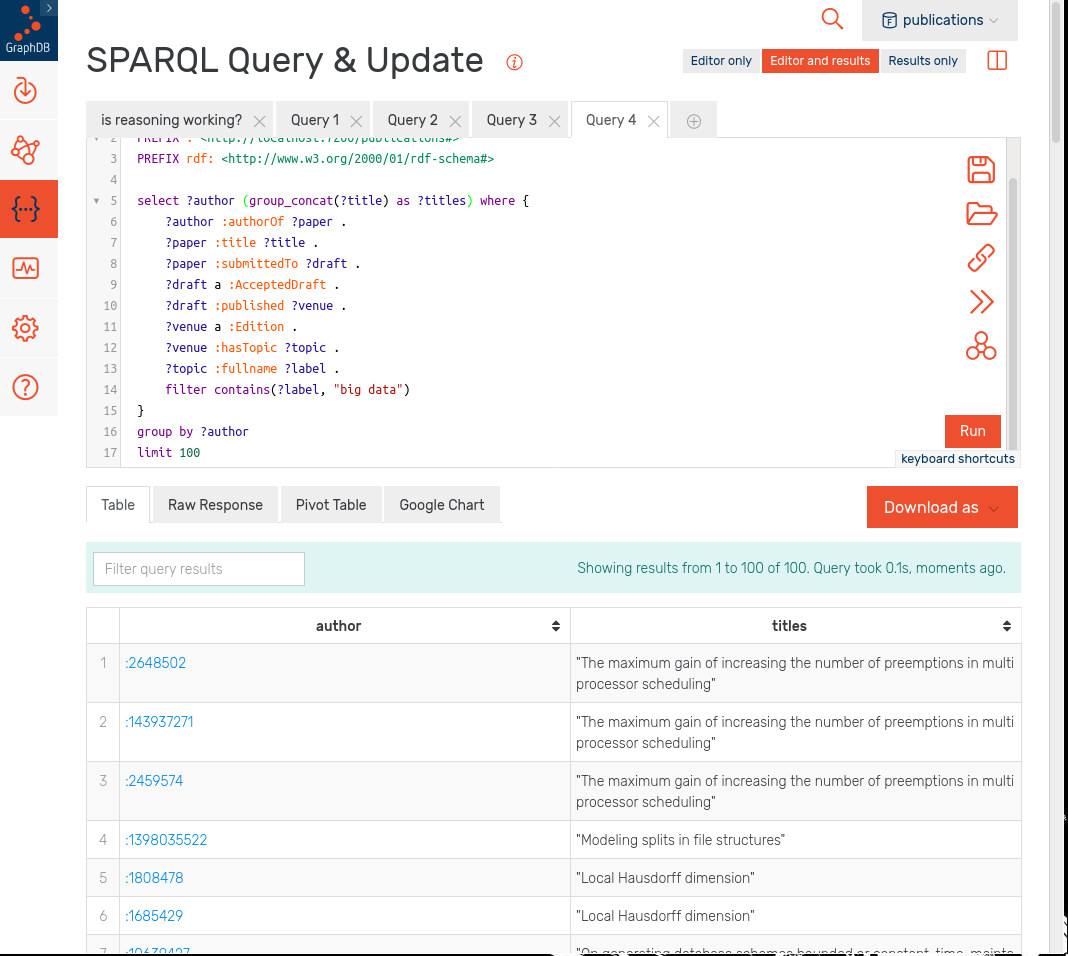
\includegraphics[width=1.0\textwidth]{query4}
  \caption{SPARQL: Query 4}
  \label{fig:query4}
\end{figure}

\begin{thebibliography}{99}

\bibitem{Owlready2} Lamy JB. \textit{Owlready: Ontology-oriented programming in Python with automatic classification and high level constructs for biomedical ontologies.} \textbf{Artificial Intelligence In Medicine 2017};80:11-28

\bibitem{DBLP} The dblp team: dblp computer science bibliography. Monthly snapshot release of March 2021.
https://dblp.org/xml/release/dblp-2021-03-01.xml.gz

\end{thebibliography}
\end{document}
